%!TEX root = ../main.tex

\chapter{Data Model}
\label{ch:data_model}

Das Data Model von \textit{Soli} ist in die Pakete \textit{dto} und \textit{domain} aufgeteilt.
Die \textit{dto}-Klassen sind die Datenübertragungsobjekte, die die Daten zwischen den Schichten des Systems übertragen.
Die \textit{domain}-Klassen sind die Datenobjekte, die in der Datenbank gespeichert werden, und bilden somit das interne Datenmodell des Systems.

Dieses Datenmodell wird mithilfe von \gls{SpringData} in der \gls{PostgreSQL}-Datenbank (welche sich zur Isolation in einem separaten \gls{Container} befindet) abgebildet.
In dieser wird das Datenmodell in Form von Tabellen und Beziehungen zwischen diesen gespeichert.
In der Anwendung werden die Datenobjekte nur im Kontext aktiver Anfragen im Arbeitsspeicher gehalten und bei Bedarf in die Datenbank geschrieben.
Als Konsequenz können die \gls{ACID}-Eigenschaften der Datenbank genutzt werden, um die Daten vor Verlust oder Inkonsistenzen zu schützen.
Damit die Daten auch über zukünftige Aktualisierungen des Systems hinweg erhalten bleiben, wird das Datenbankmigrationssystem \gls{Flyway} genutzt, der die Datenbankstruktur anpasst, wenn sich das Datenmodell ändert.

Den Kern des Buchungsmodells bildet die Klasse \hyperref[edu.kit.hci.soli.domain.Booking]{\texttt{Booking}}, die eine Buchung eines Raumes repräsentiert.
Jede Buchung ist einem Raum und einem Nutzer zugeordnet und hat einen Start- und Endzeitpunkt.
Außerdem kann eine Buchung optional einen Kommentar enthalten, der von dem Nutzer hinterlassen wurde.
Zur Umsetzung von Buchungen des Kooperationstyps \textit{ON\_REQUEST} existiert außerdem eine automatisch verwaltete Tabelle von noch offenen Anfragen für eine Buchung.

Da die Authentifikation von Nutzenden nicht durch das System selbst, sondern durch das \gls{OIDC}-System des KIT erfolgt, werden statt vollen Anmeldedaten nur die OIDC-IDs der Nutzenden gespeichert.
Diese sind im \hyperref[edu.kit.hci.soli.domain.User]{\texttt{User}}-Objekt unter dem Namen \texttt{userId} mit dem Präfix \texttt{kit/} abgelegt.
Gäste erhalten eine interne ID, welche mit dem Präfix \texttt{guest/} beginnt, und somit von den IDs der KIT-Nutzenden unterschieden werden kann.
Der Administrator des Systems hat die fixe interne ID \texttt{admin}.
Die Tabelle der Nutzenden ergänzt diese Information um die E-Mail-Adresse, den Namen, und die Sprache der Nutzenden, welche für die Kommunikation mit diesen (z.B. per E-Mail) genutzt werden.
Außerdem wird eine Flagge gespeichert, die es Administratoren ermöglicht, einzelne Nutzende zu sperren.

Eine Raumtabelle wird genutzt, um die Erweiterbarkeit des Systems zu gewährleisten.
In dieser Tabelle wird im minimalen System entsprechend der Musskriterien nur ein Raum gespeichert, welcher die ID \texttt{1} trägt.

Eine Übersicht des Datenbankmodells ist in \autoref{fig:data_model} dargestellt.

\begin{figure}[ht]
    \centering
    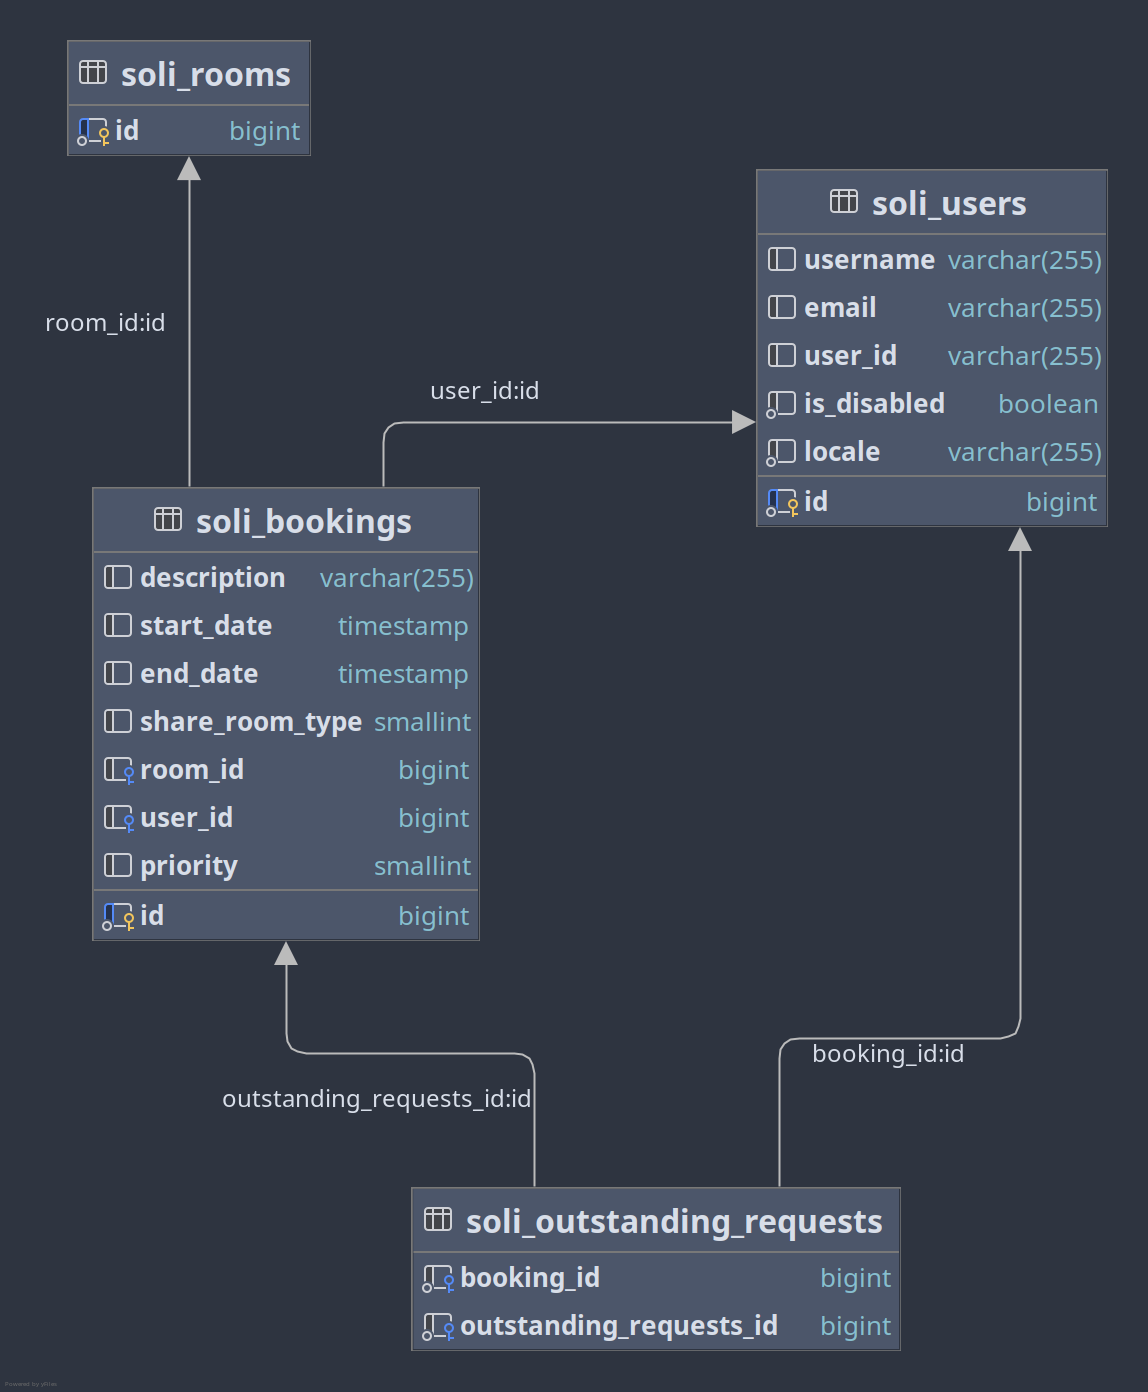
\includegraphics[width=\textwidth]{figures/database}
    \caption{Datenbankmodell von \textit{Soli}}
    \label{fig:data_model}
\end{figure}
\pagebreak



\section{Package edu.kit.hci.soli.dto}
\begin{adjustwidth}{1.5em}{0pt}
  \subsection{Interface BookingAttemptResult\label{edu.kit.hci.soli.dto.BookingAttemptResult} }
  \begin{adjustwidth}{1.5em}{0pt}
    {\begin{tabularx}{1.0\linewidth}{@{}l R@{}}
      \emph{Signature} & \texttt{public sealed abstract  interface \texttt{\hyperref[edu.kit.hci.soli.dto.BookingAttemptResult]{\texttt{BookingAttemptResult}}}} \\
      \hline
      \emph{Behaviour} & Algebraic data type representing the result of a booking attempt.  \\
      \hline
  
    \end{tabularx}}\subsubsection{Interface PossibleCooperation\label{edu.kit.hci.soli.dto.BookingAttemptResult.PossibleCooperation} }
    \begin{adjustwidth}{1.5em}{0pt}
      {\begin{tabularx}{1.0\linewidth}{@{}l R@{}}
        \emph{Signature} & \texttt{public sealed static abstract  interface \texttt{\hyperref[edu.kit.hci.soli.dto.BookingAttemptResult.PossibleCooperation]{\texttt{PossibleCooperation}} implements \texttt{\hyperref[edu.kit.hci.soli.dto.BookingAttemptResult]{\texttt{BookingAttemptResult}}}}} \\
        \hline
        \emph{Behaviour} & Algebraic data type representing a failed booking attempt that may be resolved by cooperation.  \\
        \hline
  
      \end{tabularx}}\paragraph{Method contact\label{edu.kit.hci.soli.dto.BookingAttemptResult.PossibleCooperation@contact()}}
      \begin{adjustwidth}{1.5em}{0pt}
        {\begin{tabularx}{1.0\linewidth}{@{}l R@{}}
          \emph{Signature} & \texttt{public abstract \texttt{List} contact()} \\
          \hline
          \emph{Behaviour} & Gets the list of bookings that require the permission for this cooperation. If this is not empty, the successful result of affirming this cooperation would be of type  \texttt{\hyperref[edu.kit.hci.soli.dto.BookingAttemptResult.Staged]{\texttt{Staged}}}.    \\
          \hline
          \emph{Returns} & the list of bookings to contact  \\
          \hline
  
        \end{tabularx}}
      \end{adjustwidth}\paragraph{Method cooperate\label{edu.kit.hci.soli.dto.BookingAttemptResult.PossibleCooperation@cooperate()}}
      \begin{adjustwidth}{1.5em}{0pt}
        {\begin{tabularx}{1.0\linewidth}{@{}l R@{}}
          \emph{Signature} & \texttt{public abstract \texttt{List} cooperate()} \\
          \hline
          \emph{Behaviour} & Gets the list of bookings that would happen concurrently to this booking.    \\
          \hline
          \emph{Returns} & the list of bookings to cooperate with  \\
          \hline
  
        \end{tabularx}}
      \end{adjustwidth}\paragraph{Method override\label{edu.kit.hci.soli.dto.BookingAttemptResult.PossibleCooperation@override()}}
      \begin{adjustwidth}{1.5em}{0pt}
        {\begin{tabularx}{1.0\linewidth}{@{}l R@{}}
          \emph{Signature} & \texttt{public abstract \texttt{List} override()} \\
          \hline
          \emph{Behaviour} & Gets the list of bookings that would have to be overwritten for this cooperation.    \\
          \hline
          \emph{Returns} & the list of bookings to override  \\
          \hline
  
        \end{tabularx}}
      \end{adjustwidth}\paragraph{Record Deferred\label{edu.kit.hci.soli.dto.BookingAttemptResult.PossibleCooperation.Deferred} }
      \begin{adjustwidth}{1.5em}{0pt}
        {\begin{tabularx}{1.0\linewidth}{@{}l R@{}}
          \emph{Signature} & \texttt{final public static  record \texttt{\hyperref[edu.kit.hci.soli.dto.BookingAttemptResult.PossibleCooperation.Deferred]{\texttt{Deferred}} implements \texttt{\hyperref[edu.kit.hci.soli.dto.BookingAttemptResult.PossibleCooperation]{\texttt{PossibleCooperation}}}}} \\
          \hline
          \emph{Behaviour} & Represents a deferred possible cooperation in a booking attempt. The successful result of affirming this cooperation is of type  \texttt{\hyperref[edu.kit.hci.soli.dto.BookingAttemptResult.Staged]{\texttt{Staged}}} (and, as such, will require confirmation by others).  \\
          \hline
  
        \end{tabularx}}\subparagraph{Constructor\label{edu.kit.hci.soli.dto.BookingAttemptResult.PossibleCooperation.Deferred@edu.kit.hci.soli.dto.BookingAttemptResult.PossibleCooperation.Deferred(java.util.List,java.util.List,java.util.List)}}
        \begin{adjustwidth}{1.5em}{0pt}
          {\begin{tabularx}{1.0\linewidth}{@{}l R@{}}
            \emph{Signature} & \texttt{public \texttt{\hyperref[edu.kit.hci.soli.dto.BookingAttemptResult.PossibleCooperation.Deferred]{\texttt{Deferred}}}(\texttt{List} override, \texttt{List} contact, \texttt{List} cooperate)} \\
            \hline
  
          \end{tabularx}}
        \end{adjustwidth}\subparagraph{Method override\label{edu.kit.hci.soli.dto.BookingAttemptResult.PossibleCooperation.Deferred@override()}}
        \begin{adjustwidth}{1.5em}{0pt}
          {\begin{tabularx}{1.0\linewidth}{@{}l R@{}}
            \emph{Signature} & \texttt{public \texttt{List} override()} \\
            \hline
            \emph{Behaviour} & Gets the list of bookings that would have to be overwritten for this cooperation.    \\
            \hline
            \emph{Returns} & the list of bookings to override  \\
            \hline
            \emph{Overrides} & \texttt{\texttt{\hyperref[edu.kit.hci.soli.dto.BookingAttemptResult.PossibleCooperation]{\texttt{PossibleCooperation}}}.\hyperref[edu.kit.hci.soli.dto.BookingAttemptResult$PossibleCooperation@override()]{override}\hyperref[edu.kit.hci.soli.dto.BookingAttemptResult$PossibleCooperation@override()]{(}\hyperref[edu.kit.hci.soli.dto.BookingAttemptResult$PossibleCooperation@override()]{)}} \\
            \hline
  
          \end{tabularx}}
        \end{adjustwidth}\subparagraph{Method contact\label{edu.kit.hci.soli.dto.BookingAttemptResult.PossibleCooperation.Deferred@contact()}}
        \begin{adjustwidth}{1.5em}{0pt}
          {\begin{tabularx}{1.0\linewidth}{@{}l R@{}}
            \emph{Signature} & \texttt{public \texttt{List} contact()} \\
            \hline
            \emph{Behaviour} & Gets the list of bookings that require the permission for this cooperation. If this is not empty, the successful result of affirming this cooperation would be of type  \texttt{\hyperref[edu.kit.hci.soli.dto.BookingAttemptResult.Staged]{\texttt{Staged}}}.    \\
            \hline
            \emph{Returns} & the list of bookings to contact  \\
            \hline
            \emph{Overrides} & \texttt{\texttt{\hyperref[edu.kit.hci.soli.dto.BookingAttemptResult.PossibleCooperation]{\texttt{PossibleCooperation}}}.\hyperref[edu.kit.hci.soli.dto.BookingAttemptResult$PossibleCooperation@contact()]{contact}\hyperref[edu.kit.hci.soli.dto.BookingAttemptResult$PossibleCooperation@contact()]{(}\hyperref[edu.kit.hci.soli.dto.BookingAttemptResult$PossibleCooperation@contact()]{)}} \\
            \hline
  
          \end{tabularx}}
        \end{adjustwidth}\subparagraph{Method cooperate\label{edu.kit.hci.soli.dto.BookingAttemptResult.PossibleCooperation.Deferred@cooperate()}}
        \begin{adjustwidth}{1.5em}{0pt}
          {\begin{tabularx}{1.0\linewidth}{@{}l R@{}}
            \emph{Signature} & \texttt{public \texttt{List} cooperate()} \\
            \hline
            \emph{Behaviour} & Gets the list of bookings that would happen concurrently to this booking.    \\
            \hline
            \emph{Returns} & the list of bookings to cooperate with  \\
            \hline
            \emph{Overrides} & \texttt{\texttt{\hyperref[edu.kit.hci.soli.dto.BookingAttemptResult.PossibleCooperation]{\texttt{PossibleCooperation}}}.\hyperref[edu.kit.hci.soli.dto.BookingAttemptResult$PossibleCooperation@cooperate()]{cooperate}\hyperref[edu.kit.hci.soli.dto.BookingAttemptResult$PossibleCooperation@cooperate()]{(}\hyperref[edu.kit.hci.soli.dto.BookingAttemptResult$PossibleCooperation@cooperate()]{)}} \\
            \hline
  
          \end{tabularx}}
        \end{adjustwidth}
      \end{adjustwidth}\paragraph{Record Immediate\label{edu.kit.hci.soli.dto.BookingAttemptResult.PossibleCooperation.Immediate} }
      \begin{adjustwidth}{1.5em}{0pt}
        {\begin{tabularx}{1.0\linewidth}{@{}l R@{}}
          \emph{Signature} & \texttt{final public static  record \texttt{\hyperref[edu.kit.hci.soli.dto.BookingAttemptResult.PossibleCooperation.Immediate]{\texttt{Immediate}} implements \texttt{\hyperref[edu.kit.hci.soli.dto.BookingAttemptResult.PossibleCooperation]{\texttt{PossibleCooperation}}}}} \\
          \hline
          \emph{Behaviour} & Represents an immediate possible cooperation in a booking attempt. The successful result of affirming this cooperation is an immediate  \texttt{\hyperref[edu.kit.hci.soli.dto.BookingAttemptResult.Success]{\texttt{Success}}}.  \\
          \hline
  
        \end{tabularx}}\subparagraph{Constructor\label{edu.kit.hci.soli.dto.BookingAttemptResult.PossibleCooperation.Immediate@edu.kit.hci.soli.dto.BookingAttemptResult.PossibleCooperation.Immediate(java.util.List,java.util.List)}}
        \begin{adjustwidth}{1.5em}{0pt}
          {\begin{tabularx}{1.0\linewidth}{@{}l R@{}}
            \emph{Signature} & \texttt{public \texttt{\hyperref[edu.kit.hci.soli.dto.BookingAttemptResult.PossibleCooperation.Immediate]{\texttt{Immediate}}}(\texttt{List} override, \texttt{List} cooperate)} \\
            \hline
  
          \end{tabularx}}
        \end{adjustwidth}\subparagraph{Method contact\label{edu.kit.hci.soli.dto.BookingAttemptResult.PossibleCooperation.Immediate@contact()}}
        \begin{adjustwidth}{1.5em}{0pt}
          {\begin{tabularx}{1.0\linewidth}{@{}l R@{}}
            \emph{Signature} & \texttt{public \texttt{List} contact()} \\
            \hline
            \emph{Behaviour} & Gets the list of bookings that require the permission for this cooperation. If this is not empty, the successful result of affirming this cooperation would be of type  \texttt{\hyperref[edu.kit.hci.soli.dto.BookingAttemptResult.Staged]{\texttt{Staged}}}.    \\
            \hline
            \emph{Returns} & the list of bookings to contact  \\
            \hline
            \emph{Overrides} & \texttt{\texttt{\hyperref[edu.kit.hci.soli.dto.BookingAttemptResult.PossibleCooperation]{\texttt{PossibleCooperation}}}.\hyperref[edu.kit.hci.soli.dto.BookingAttemptResult$PossibleCooperation@contact()]{contact}\hyperref[edu.kit.hci.soli.dto.BookingAttemptResult$PossibleCooperation@contact()]{(}\hyperref[edu.kit.hci.soli.dto.BookingAttemptResult$PossibleCooperation@contact()]{)}} \\
            \hline
  
          \end{tabularx}}
        \end{adjustwidth}\subparagraph{Method override\label{edu.kit.hci.soli.dto.BookingAttemptResult.PossibleCooperation.Immediate@override()}}
        \begin{adjustwidth}{1.5em}{0pt}
          {\begin{tabularx}{1.0\linewidth}{@{}l R@{}}
            \emph{Signature} & \texttt{public \texttt{List} override()} \\
            \hline
            \emph{Behaviour} & Gets the list of bookings that would have to be overwritten for this cooperation.    \\
            \hline
            \emph{Returns} & the list of bookings to override  \\
            \hline
            \emph{Overrides} & \texttt{\texttt{\hyperref[edu.kit.hci.soli.dto.BookingAttemptResult.PossibleCooperation]{\texttt{PossibleCooperation}}}.\hyperref[edu.kit.hci.soli.dto.BookingAttemptResult$PossibleCooperation@override()]{override}\hyperref[edu.kit.hci.soli.dto.BookingAttemptResult$PossibleCooperation@override()]{(}\hyperref[edu.kit.hci.soli.dto.BookingAttemptResult$PossibleCooperation@override()]{)}} \\
            \hline
  
          \end{tabularx}}
        \end{adjustwidth}\subparagraph{Method cooperate\label{edu.kit.hci.soli.dto.BookingAttemptResult.PossibleCooperation.Immediate@cooperate()}}
        \begin{adjustwidth}{1.5em}{0pt}
          {\begin{tabularx}{1.0\linewidth}{@{}l R@{}}
            \emph{Signature} & \texttt{public \texttt{List} cooperate()} \\
            \hline
            \emph{Behaviour} & Gets the list of bookings that would happen concurrently to this booking.    \\
            \hline
            \emph{Returns} & the list of bookings to cooperate with  \\
            \hline
            \emph{Overrides} & \texttt{\texttt{\hyperref[edu.kit.hci.soli.dto.BookingAttemptResult.PossibleCooperation]{\texttt{PossibleCooperation}}}.\hyperref[edu.kit.hci.soli.dto.BookingAttemptResult$PossibleCooperation@cooperate()]{cooperate}\hyperref[edu.kit.hci.soli.dto.BookingAttemptResult$PossibleCooperation@cooperate()]{(}\hyperref[edu.kit.hci.soli.dto.BookingAttemptResult$PossibleCooperation@cooperate()]{)}} \\
            \hline
  
          \end{tabularx}}
        \end{adjustwidth}
      \end{adjustwidth}
    \end{adjustwidth}\subsubsection{Record Failure\label{edu.kit.hci.soli.dto.BookingAttemptResult.Failure} }
    \begin{adjustwidth}{1.5em}{0pt}
      {\begin{tabularx}{1.0\linewidth}{@{}l R@{}}
        \emph{Signature} & \texttt{final public static  record \texttt{\hyperref[edu.kit.hci.soli.dto.BookingAttemptResult.Failure]{\texttt{Failure}} implements \texttt{\hyperref[edu.kit.hci.soli.dto.BookingAttemptResult]{\texttt{BookingAttemptResult}}}}} \\
        \hline
        \emph{Behaviour} & Represents a booking attempt that has failed because of an unresolveable conflict with a booking of higher or equal priority.  \\
        \hline
  
      \end{tabularx}}\paragraph{Constructor\label{edu.kit.hci.soli.dto.BookingAttemptResult.Failure@edu.kit.hci.soli.dto.BookingAttemptResult.Failure(java.util.List)}}
      \begin{adjustwidth}{1.5em}{0pt}
        {\begin{tabularx}{1.0\linewidth}{@{}l R@{}}
          \emph{Signature} & \texttt{public \texttt{\hyperref[edu.kit.hci.soli.dto.BookingAttemptResult.Failure]{\texttt{Failure}}}(\texttt{List} conflict)} \\
          \hline
  
        \end{tabularx}}
      \end{adjustwidth}\paragraph{Method conflict\label{edu.kit.hci.soli.dto.BookingAttemptResult.Failure@conflict()}}
      \begin{adjustwidth}{1.5em}{0pt}
        {\begin{tabularx}{1.0\linewidth}{@{}l R@{}}
          \emph{Signature} & \texttt{public \texttt{List} conflict()} \\
          \hline
  
        \end{tabularx}}
      \end{adjustwidth}
    \end{adjustwidth}\subsubsection{Record Staged\label{edu.kit.hci.soli.dto.BookingAttemptResult.Staged} }
    \begin{adjustwidth}{1.5em}{0pt}
      {\begin{tabularx}{1.0\linewidth}{@{}l R@{}}
        \emph{Signature} & \texttt{final public static  record \texttt{\hyperref[edu.kit.hci.soli.dto.BookingAttemptResult.Staged]{\texttt{Staged}} implements \texttt{\hyperref[edu.kit.hci.soli.dto.BookingAttemptResult]{\texttt{BookingAttemptResult}}}}} \\
        \hline
        \emph{Behaviour} & Represents a booking attempt that was successful but requires confirmation by one or more users.  \\
        \hline
  
      \end{tabularx}}\paragraph{Constructor\label{edu.kit.hci.soli.dto.BookingAttemptResult.Staged@edu.kit.hci.soli.dto.BookingAttemptResult.Staged(edu.kit.hci.soli.domain.Booking)}}
      \begin{adjustwidth}{1.5em}{0pt}
        {\begin{tabularx}{1.0\linewidth}{@{}l R@{}}
          \emph{Signature} & \texttt{public \texttt{\hyperref[edu.kit.hci.soli.dto.BookingAttemptResult.Staged]{\texttt{Staged}}}(\texttt{\hyperref[edu.kit.hci.soli.domain.Booking]{\texttt{Booking}}} booking)} \\
          \hline
  
        \end{tabularx}}
      \end{adjustwidth}\paragraph{Method booking\label{edu.kit.hci.soli.dto.BookingAttemptResult.Staged@booking()}}
      \begin{adjustwidth}{1.5em}{0pt}
        {\begin{tabularx}{1.0\linewidth}{@{}l R@{}}
          \emph{Signature} & \texttt{public \texttt{\hyperref[edu.kit.hci.soli.domain.Booking]{\texttt{Booking}}} booking()} \\
          \hline
  
        \end{tabularx}}
      \end{adjustwidth}
    \end{adjustwidth}\subsubsection{Record Success\label{edu.kit.hci.soli.dto.BookingAttemptResult.Success} }
    \begin{adjustwidth}{1.5em}{0pt}
      {\begin{tabularx}{1.0\linewidth}{@{}l R@{}}
        \emph{Signature} & \texttt{final public static  record \texttt{\hyperref[edu.kit.hci.soli.dto.BookingAttemptResult.Success]{\texttt{Success}} implements \texttt{\hyperref[edu.kit.hci.soli.dto.BookingAttemptResult]{\texttt{BookingAttemptResult}}}}} \\
        \hline
        \emph{Behaviour} & Represents a successful booking attempt.  \\
        \hline
  
      \end{tabularx}}\paragraph{Constructor\label{edu.kit.hci.soli.dto.BookingAttemptResult.Success@edu.kit.hci.soli.dto.BookingAttemptResult.Success(edu.kit.hci.soli.domain.Booking)}}
      \begin{adjustwidth}{1.5em}{0pt}
        {\begin{tabularx}{1.0\linewidth}{@{}l R@{}}
          \emph{Signature} & \texttt{public \texttt{\hyperref[edu.kit.hci.soli.dto.BookingAttemptResult.Success]{\texttt{Success}}}(\texttt{\hyperref[edu.kit.hci.soli.domain.Booking]{\texttt{Booking}}} booking)} \\
          \hline
  
        \end{tabularx}}
      \end{adjustwidth}\paragraph{Method booking\label{edu.kit.hci.soli.dto.BookingAttemptResult.Success@booking()}}
      \begin{adjustwidth}{1.5em}{0pt}
        {\begin{tabularx}{1.0\linewidth}{@{}l R@{}}
          \emph{Signature} & \texttt{public \texttt{\hyperref[edu.kit.hci.soli.domain.Booking]{\texttt{Booking}}} booking()} \\
          \hline
  
        \end{tabularx}}
      \end{adjustwidth}
    \end{adjustwidth}
  \end{adjustwidth}\subsection{Enum BookingDeleteReason\label{edu.kit.hci.soli.dto.BookingDeleteReason} }
  \begin{adjustwidth}{1.5em}{0pt}
    {\begin{tabularx}{1.0\linewidth}{@{}l R@{}}
      \emph{Signature} & \texttt{final public  enum \texttt{\hyperref[edu.kit.hci.soli.dto.BookingDeleteReason]{\texttt{BookingDeleteReason}}}} \\
      \hline
      \emph{Behaviour} & Enumeration representing the reasons for deleting a booking.  \\
      \hline
  
    \end{tabularx}}
  \end{adjustwidth}\subsection{Record CalendarEvent\label{edu.kit.hci.soli.dto.CalendarEvent} }
  \begin{adjustwidth}{1.5em}{0pt}
    {\begin{tabularx}{1.0\linewidth}{@{}l R@{}}
      \emph{Signature} & \texttt{final public  record \texttt{\hyperref[edu.kit.hci.soli.dto.CalendarEvent]{\texttt{CalendarEvent}}}} \\
      \hline
      \emph{Behaviour} & Record representing an event as specified by FullCalendar.    \\
      \hline
      \emph{Parameters} & {\begin{tabularx}{1.0\linewidth}{@{}l R@{}}
        \texttt{url}: &        the URL associated with the event  \\
        \texttt{title}: &      the title of the event  \\
        \texttt{start}: &      the start date and time of the event  \\
        \texttt{end}: &        the end date and time of the event  \\
        \texttt{classNames}: & the list of CSS classes to use for the generated HTML element of this event  \\
  
      \end{tabularx}} \\
      \hline
  
    \end{tabularx}}\subsubsection{Constructor\label{edu.kit.hci.soli.dto.CalendarEvent@edu.kit.hci.soli.dto.CalendarEvent(java.lang.String,java.lang.String,java.time.LocalDateTime,java.time.LocalDateTime,java.util.List)}}
    \begin{adjustwidth}{1.5em}{0pt}
      {\begin{tabularx}{1.0\linewidth}{@{}l R@{}}
        \emph{Signature} & \texttt{public \texttt{\hyperref[edu.kit.hci.soli.dto.CalendarEvent]{\texttt{CalendarEvent}}}(\texttt{String} url, \texttt{String} title, \texttt{LocalDateTime} start, \texttt{LocalDateTime} end, \texttt{List} classNames)} \\
        \hline
  
      \end{tabularx}}
    \end{adjustwidth}\subsubsection{Method url\label{edu.kit.hci.soli.dto.CalendarEvent@url()}}
    \begin{adjustwidth}{1.5em}{0pt}
      {\begin{tabularx}{1.0\linewidth}{@{}l R@{}}
        \emph{Signature} & \texttt{public \texttt{String} url()} \\
        \hline
  
      \end{tabularx}}
    \end{adjustwidth}\subsubsection{Method title\label{edu.kit.hci.soli.dto.CalendarEvent@title()}}
    \begin{adjustwidth}{1.5em}{0pt}
      {\begin{tabularx}{1.0\linewidth}{@{}l R@{}}
        \emph{Signature} & \texttt{public \texttt{String} title()} \\
        \hline
  
      \end{tabularx}}
    \end{adjustwidth}\subsubsection{Method start\label{edu.kit.hci.soli.dto.CalendarEvent@start()}}
    \begin{adjustwidth}{1.5em}{0pt}
      {\begin{tabularx}{1.0\linewidth}{@{}l R@{}}
        \emph{Signature} & \texttt{public \texttt{LocalDateTime} start()} \\
        \hline
  
      \end{tabularx}}
    \end{adjustwidth}\subsubsection{Method end\label{edu.kit.hci.soli.dto.CalendarEvent@end()}}
    \begin{adjustwidth}{1.5em}{0pt}
      {\begin{tabularx}{1.0\linewidth}{@{}l R@{}}
        \emph{Signature} & \texttt{public \texttt{LocalDateTime} end()} \\
        \hline
  
      \end{tabularx}}
    \end{adjustwidth}\subsubsection{Method classNames\label{edu.kit.hci.soli.dto.CalendarEvent@classNames()}}
    \begin{adjustwidth}{1.5em}{0pt}
      {\begin{tabularx}{1.0\linewidth}{@{}l R@{}}
        \emph{Signature} & \texttt{public \texttt{List} classNames()} \\
        \hline
  
      \end{tabularx}}
    \end{adjustwidth}
  \end{adjustwidth}\subsection{Enum KnownError\label{edu.kit.hci.soli.dto.KnownError} }
  \begin{adjustwidth}{1.5em}{0pt}
    {\begin{tabularx}{1.0\linewidth}{@{}l R@{}}
      \emph{Signature} & \texttt{final public  enum \texttt{\hyperref[edu.kit.hci.soli.dto.KnownError]{\texttt{KnownError}}}} \\
      \hline
      \emph{Behaviour} & Enumeration representing known errors with their corresponding titles and messages.  \\
      \hline
  
    \end{tabularx}}\subsubsection{Field message\label{edu.kit.hci.soli.dto.KnownError@message}}
    \begin{adjustwidth}{1.5em}{0pt}
      {\begin{tabularx}{1.0\linewidth}{@{}l R@{}}
        \emph{Signature} & \texttt{final public \texttt{\hyperref[edu.kit.hci.soli.dto.KnownError]{\texttt{KnownError}}} message} \\
        \hline
        \emph{Behaviour} & The detailed error message.  \\
        \hline
  
      \end{tabularx}}
    \end{adjustwidth}\subsubsection{Field title\label{edu.kit.hci.soli.dto.KnownError@title}}
    \begin{adjustwidth}{1.5em}{0pt}
      {\begin{tabularx}{1.0\linewidth}{@{}l R@{}}
        \emph{Signature} & \texttt{final public \texttt{\hyperref[edu.kit.hci.soli.dto.KnownError]{\texttt{KnownError}}} title} \\
        \hline
        \emph{Behaviour} & The title of the error message.  \\
        \hline
  
      \end{tabularx}}
    \end{adjustwidth}
  \end{adjustwidth}\subsection{Record LoginStateModel\label{edu.kit.hci.soli.dto.LoginStateModel} }
  \begin{adjustwidth}{1.5em}{0pt}
    {\begin{tabularx}{1.0\linewidth}{@{}l R@{}}
      \emph{Signature} & \texttt{final public  record \texttt{\hyperref[edu.kit.hci.soli.dto.LoginStateModel]{\texttt{LoginStateModel}}}} \\
      \hline
      \emph{Behaviour} & Record representing the login state model.    \\
      \hline
      \emph{Parameters} & {\begin{tabularx}{1.0\linewidth}{@{}l R@{}}
        \texttt{name}: &      the name of the user  \\
        \texttt{kind}: &      the kind of login  \\
        \texttt{csrfToken}: & the CSRF token associated with the login  \\
        \texttt{user}: &      the user associated with the login, can be null  \\
  
      \end{tabularx}} \\
      \hline
  
    \end{tabularx}}\subsubsection{Constructor\label{edu.kit.hci.soli.dto.LoginStateModel@edu.kit.hci.soli.dto.LoginStateModel(java.lang.String,edu.kit.hci.soli.dto.LoginStateModel.Kind,org.springframework.security.web.csrf.CsrfToken,edu.kit.hci.soli.domain.User)}}
    \begin{adjustwidth}{1.5em}{0pt}
      {\begin{tabularx}{1.0\linewidth}{@{}l R@{}}
        \emph{Signature} & \texttt{public \texttt{\hyperref[edu.kit.hci.soli.dto.LoginStateModel]{\texttt{LoginStateModel}}}(\texttt{String} name, \texttt{\hyperref[edu.kit.hci.soli.dto.LoginStateModel.Kind]{\texttt{Kind}}} kind, \texttt{CsrfToken} csrfToken, \texttt{\hyperref[edu.kit.hci.soli.domain.User]{\texttt{User}}} user)} \\
        \hline
  
      \end{tabularx}}
    \end{adjustwidth}\subsubsection{Method name\label{edu.kit.hci.soli.dto.LoginStateModel@name()}}
    \begin{adjustwidth}{1.5em}{0pt}
      {\begin{tabularx}{1.0\linewidth}{@{}l R@{}}
        \emph{Signature} & \texttt{public \texttt{String} name()} \\
        \hline
  
      \end{tabularx}}
    \end{adjustwidth}\subsubsection{Method kind\label{edu.kit.hci.soli.dto.LoginStateModel@kind()}}
    \begin{adjustwidth}{1.5em}{0pt}
      {\begin{tabularx}{1.0\linewidth}{@{}l R@{}}
        \emph{Signature} & \texttt{public \texttt{\hyperref[edu.kit.hci.soli.dto.LoginStateModel.Kind]{\texttt{Kind}}} kind()} \\
        \hline
  
      \end{tabularx}}
    \end{adjustwidth}\subsubsection{Method csrfToken\label{edu.kit.hci.soli.dto.LoginStateModel@csrfToken()}}
    \begin{adjustwidth}{1.5em}{0pt}
      {\begin{tabularx}{1.0\linewidth}{@{}l R@{}}
        \emph{Signature} & \texttt{public \texttt{CsrfToken} csrfToken()} \\
        \hline
  
      \end{tabularx}}
    \end{adjustwidth}\subsubsection{Method user\label{edu.kit.hci.soli.dto.LoginStateModel@user()}}
    \begin{adjustwidth}{1.5em}{0pt}
      {\begin{tabularx}{1.0\linewidth}{@{}l R@{}}
        \emph{Signature} & \texttt{public \texttt{\hyperref[edu.kit.hci.soli.domain.User]{\texttt{User}}} user()} \\
        \hline
  
      \end{tabularx}}
    \end{adjustwidth}\subsubsection{Enum Kind\label{edu.kit.hci.soli.dto.LoginStateModel.Kind} }
    \begin{adjustwidth}{1.5em}{0pt}
      {\begin{tabularx}{1.0\linewidth}{@{}l R@{}}
        \emph{Signature} & \texttt{final public static  enum \texttt{\hyperref[edu.kit.hci.soli.dto.LoginStateModel.Kind]{\texttt{Kind}}}} \\
        \hline
        \emph{Behaviour} & Enumeration representing the kind of login.  \\
        \hline
  
      \end{tabularx}}
    \end{adjustwidth}
  \end{adjustwidth}
\end{adjustwidth}


\section{Package edu.kit.hci.soli.domain}
\begin{adjustwidth}{1.5em}{0pt}
  \subsection{Class Booking\label{edu.kit.hci.soli.domain.Booking} }
  \begin{adjustwidth}{1.5em}{0pt}
    {\begin{tabularx}{1.0\linewidth}{@{}l R@{}}
      \emph{Signature} & \texttt{public  class \texttt{\hyperref[edu.kit.hci.soli.domain.Booking]{\texttt{Booking}}}} \\
      \hline
      \emph{Behaviour} & The datamodel for a Booking as it is stored in the database.  \\
      \hline
  
    \end{tabularx}}\subsubsection{Constructor\label{edu.kit.hci.soli.domain.Booking@edu.kit.hci.soli.domain.Booking()}}
    \begin{adjustwidth}{1.5em}{0pt}
      {\begin{tabularx}{1.0\linewidth}{@{}l R@{}}
        \emph{Signature} & \texttt{public \texttt{\hyperref[edu.kit.hci.soli.domain.Booking]{\texttt{Booking}}}()} \\
        \hline
        \emph{Behaviour} & Default constructor for Booking.  \\
        \hline
  
      \end{tabularx}}
    \end{adjustwidth}\subsubsection{Constructor\label{edu.kit.hci.soli.domain.Booking@edu.kit.hci.soli.domain.Booking(java.lang.Long,java.lang.String,java.time.LocalDateTime,java.time.LocalDateTime,edu.kit.hci.soli.domain.ShareRoomType,edu.kit.hci.soli.domain.Room,edu.kit.hci.soli.domain.User,edu.kit.hci.soli.domain.Priority,java.util.Set)}}
    \begin{adjustwidth}{1.5em}{0pt}
      {\begin{tabularx}{1.0\linewidth}{@{}l R@{}}
        \emph{Signature} & \texttt{public \texttt{\hyperref[edu.kit.hci.soli.domain.Booking]{\texttt{Booking}}}(\texttt{Long} id, \texttt{String} description, \texttt{LocalDateTime} startDate, \texttt{LocalDateTime} endDate, \texttt{\hyperref[edu.kit.hci.soli.domain.ShareRoomType]{\texttt{ShareRoomType}}} shareRoomType, \texttt{\hyperref[edu.kit.hci.soli.domain.Room]{\texttt{Room}}} room, \texttt{\hyperref[edu.kit.hci.soli.domain.User]{\texttt{User}}} user, \texttt{\hyperref[edu.kit.hci.soli.domain.Priority]{\texttt{Priority}}} priority, \texttt{Set} openRequests)} \\
        \hline
        \emph{Behaviour} & Constructs a new Booking with the specified details.    \\
        \hline
        \emph{Parameters} & {\begin{tabularx}{1.0\linewidth}{@{}l R@{}}
          \texttt{id}: &                  the unique identifier for the booking  \\
          \texttt{description}: &         a description of the booking  \\
          \texttt{startDate}: &           the start date and time of the booking  \\
          \texttt{endDate}: &             the end date and time of the booking  \\
          \texttt{shareRoomType}: &       the kind of room sharing for the booking  \\
          \texttt{room}: &                the room associated with the booking  \\
          \texttt{user}: &                the user who made the booking  \\
          \texttt{priority}: &            the priority level of the booking  \\
          \texttt{openRequests}: & the set of share requests that must still be resolved  \\
  
        \end{tabularx}} \\
        \hline
  
      \end{tabularx}}
    \end{adjustwidth}\subsubsection{Method hashCode\label{edu.kit.hci.soli.domain.Booking@hashCode()}}
    \begin{adjustwidth}{1.5em}{0pt}
      {\begin{tabularx}{1.0\linewidth}{@{}l R@{}}
        \emph{Signature} & \texttt{public \texttt{int} hashCode()} \\
        \hline
  
      \end{tabularx}}
    \end{adjustwidth}\subsubsection{Method equals\label{edu.kit.hci.soli.domain.Booking@equals(java.lang.Object)}}
    \begin{adjustwidth}{1.5em}{0pt}
      {\begin{tabularx}{1.0\linewidth}{@{}l R@{}}
        \emph{Signature} & \texttt{public \texttt{boolean} equals(\texttt{Object} o)} \\
        \hline
  
      \end{tabularx}}
    \end{adjustwidth}\subsubsection{Method setOpenRequests\label{edu.kit.hci.soli.domain.Booking@setOpenRequests(java.util.Set)}}
    \begin{adjustwidth}{1.5em}{0pt}
      {\begin{tabularx}{1.0\linewidth}{@{}l R@{}}
        \emph{Signature} & \texttt{public \texttt{void} setOpenRequests(\texttt{Set} openRequests)} \\
        \hline
        \emph{Behaviour} & Sets the set of share requests that must still be resolved for this booking to be confirmed.    \\
        \hline
        \emph{Parameters} & {\begin{tabularx}{1.0\linewidth}{@{}l R@{}}
          \texttt{openRequests}: & the set of share requests that must still be resolved  \\
  
        \end{tabularx}} \\
        \hline
  
      \end{tabularx}}
    \end{adjustwidth}\subsubsection{Method setPriority\label{edu.kit.hci.soli.domain.Booking@setPriority(edu.kit.hci.soli.domain.Priority)}}
    \begin{adjustwidth}{1.5em}{0pt}
      {\begin{tabularx}{1.0\linewidth}{@{}l R@{}}
        \emph{Signature} & \texttt{public \texttt{void} setPriority(\texttt{\hyperref[edu.kit.hci.soli.domain.Priority]{\texttt{Priority}}} priority)} \\
        \hline
        \emph{Behaviour} & Sets the priority level of the booking.    \\
        \hline
        \emph{Parameters} & {\begin{tabularx}{1.0\linewidth}{@{}l R@{}}
          \texttt{priority}: & the priority level of the booking  \\
  
        \end{tabularx}} \\
        \hline
  
      \end{tabularx}}
    \end{adjustwidth}\subsubsection{Method setUser\label{edu.kit.hci.soli.domain.Booking@setUser(edu.kit.hci.soli.domain.User)}}
    \begin{adjustwidth}{1.5em}{0pt}
      {\begin{tabularx}{1.0\linewidth}{@{}l R@{}}
        \emph{Signature} & \texttt{public \texttt{void} setUser(\texttt{\hyperref[edu.kit.hci.soli.domain.User]{\texttt{User}}} user)} \\
        \hline
        \emph{Behaviour} & Sets the user who made the booking.    \\
        \hline
        \emph{Parameters} & {\begin{tabularx}{1.0\linewidth}{@{}l R@{}}
          \texttt{user}: & the user who made the booking  \\
  
        \end{tabularx}} \\
        \hline
  
      \end{tabularx}}
    \end{adjustwidth}\subsubsection{Method setRoom\label{edu.kit.hci.soli.domain.Booking@setRoom(edu.kit.hci.soli.domain.Room)}}
    \begin{adjustwidth}{1.5em}{0pt}
      {\begin{tabularx}{1.0\linewidth}{@{}l R@{}}
        \emph{Signature} & \texttt{public \texttt{void} setRoom(\texttt{\hyperref[edu.kit.hci.soli.domain.Room]{\texttt{Room}}} room)} \\
        \hline
        \emph{Behaviour} & Sets the room associated with the booking.    \\
        \hline
        \emph{Parameters} & {\begin{tabularx}{1.0\linewidth}{@{}l R@{}}
          \texttt{room}: & the room associated with the booking  \\
  
        \end{tabularx}} \\
        \hline
  
      \end{tabularx}}
    \end{adjustwidth}\subsubsection{Method setShareRoomType\label{edu.kit.hci.soli.domain.Booking@setShareRoomType(edu.kit.hci.soli.domain.ShareRoomType)}}
    \begin{adjustwidth}{1.5em}{0pt}
      {\begin{tabularx}{1.0\linewidth}{@{}l R@{}}
        \emph{Signature} & \texttt{public \texttt{void} setShareRoomType(\texttt{\hyperref[edu.kit.hci.soli.domain.ShareRoomType]{\texttt{ShareRoomType}}} shareRoomType)} \\
        \hline
        \emph{Behaviour} & Sets the kind of room sharing for the booking.    \\
        \hline
        \emph{Parameters} & {\begin{tabularx}{1.0\linewidth}{@{}l R@{}}
          \texttt{shareRoomType}: & the kind of room sharing for the booking  \\
  
        \end{tabularx}} \\
        \hline
  
      \end{tabularx}}
    \end{adjustwidth}\subsubsection{Method setEndDate\label{edu.kit.hci.soli.domain.Booking@setEndDate(java.time.LocalDateTime)}}
    \begin{adjustwidth}{1.5em}{0pt}
      {\begin{tabularx}{1.0\linewidth}{@{}l R@{}}
        \emph{Signature} & \texttt{public \texttt{void} setEndDate(\texttt{LocalDateTime} endDate)} \\
        \hline
        \emph{Behaviour} & Sets the end date and time of the booking.    \\
        \hline
        \emph{Parameters} & {\begin{tabularx}{1.0\linewidth}{@{}l R@{}}
          \texttt{endDate}: & the end date and time of the booking  \\
  
        \end{tabularx}} \\
        \hline
  
      \end{tabularx}}
    \end{adjustwidth}\subsubsection{Method setStartDate\label{edu.kit.hci.soli.domain.Booking@setStartDate(java.time.LocalDateTime)}}
    \begin{adjustwidth}{1.5em}{0pt}
      {\begin{tabularx}{1.0\linewidth}{@{}l R@{}}
        \emph{Signature} & \texttt{public \texttt{void} setStartDate(\texttt{LocalDateTime} startDate)} \\
        \hline
        \emph{Behaviour} & Sets the start date and time of the booking.    \\
        \hline
        \emph{Parameters} & {\begin{tabularx}{1.0\linewidth}{@{}l R@{}}
          \texttt{startDate}: & the start date and time of the booking  \\
  
        \end{tabularx}} \\
        \hline
  
      \end{tabularx}}
    \end{adjustwidth}\subsubsection{Method setDescription\label{edu.kit.hci.soli.domain.Booking@setDescription(java.lang.String)}}
    \begin{adjustwidth}{1.5em}{0pt}
      {\begin{tabularx}{1.0\linewidth}{@{}l R@{}}
        \emph{Signature} & \texttt{public \texttt{void} setDescription(\texttt{String} description)} \\
        \hline
        \emph{Behaviour} & Sets the description of the booking.    \\
        \hline
        \emph{Parameters} & {\begin{tabularx}{1.0\linewidth}{@{}l R@{}}
          \texttt{description}: & the description of the booking  \\
  
        \end{tabularx}} \\
        \hline
  
      \end{tabularx}}
    \end{adjustwidth}\subsubsection{Method setId\label{edu.kit.hci.soli.domain.Booking@setId(java.lang.Long)}}
    \begin{adjustwidth}{1.5em}{0pt}
      {\begin{tabularx}{1.0\linewidth}{@{}l R@{}}
        \emph{Signature} & \texttt{public \texttt{void} setId(\texttt{Long} id)} \\
        \hline
        \emph{Behaviour} & Sets the unique identifier for the booking.    \\
        \hline
        \emph{Parameters} & {\begin{tabularx}{1.0\linewidth}{@{}l R@{}}
          \texttt{id}: & the unique identifier for the booking  \\
  
        \end{tabularx}} \\
        \hline
  
      \end{tabularx}}
    \end{adjustwidth}\subsubsection{Method getOpenRequests\label{edu.kit.hci.soli.domain.Booking@getOpenRequests()}}
    \begin{adjustwidth}{1.5em}{0pt}
      {\begin{tabularx}{1.0\linewidth}{@{}l R@{}}
        \emph{Signature} & \texttt{public \texttt{Set} getOpenRequests()} \\
        \hline
        \emph{Behaviour} & Gets the set of share requests that must still be resolved for this booking to be confirmed.    \\
        \hline
        \emph{Returns} & the set of share requests that must still be resolved  \\
        \hline
  
      \end{tabularx}}
    \end{adjustwidth}\subsubsection{Method getPriority\label{edu.kit.hci.soli.domain.Booking@getPriority()}}
    \begin{adjustwidth}{1.5em}{0pt}
      {\begin{tabularx}{1.0\linewidth}{@{}l R@{}}
        \emph{Signature} & \texttt{public \texttt{\hyperref[edu.kit.hci.soli.domain.Priority]{\texttt{Priority}}} getPriority()} \\
        \hline
        \emph{Behaviour} & Gets the priority level of the booking.    \\
        \hline
        \emph{Returns} & the priority level of the booking  \\
        \hline
  
      \end{tabularx}}
    \end{adjustwidth}\subsubsection{Method getUser\label{edu.kit.hci.soli.domain.Booking@getUser()}}
    \begin{adjustwidth}{1.5em}{0pt}
      {\begin{tabularx}{1.0\linewidth}{@{}l R@{}}
        \emph{Signature} & \texttt{public \texttt{\hyperref[edu.kit.hci.soli.domain.User]{\texttt{User}}} getUser()} \\
        \hline
        \emph{Behaviour} & Gets the user who made the booking.    \\
        \hline
        \emph{Returns} & the user who made the booking  \\
        \hline
  
      \end{tabularx}}
    \end{adjustwidth}\subsubsection{Method getRoom\label{edu.kit.hci.soli.domain.Booking@getRoom()}}
    \begin{adjustwidth}{1.5em}{0pt}
      {\begin{tabularx}{1.0\linewidth}{@{}l R@{}}
        \emph{Signature} & \texttt{public \texttt{\hyperref[edu.kit.hci.soli.domain.Room]{\texttt{Room}}} getRoom()} \\
        \hline
        \emph{Behaviour} & Gets the room associated with the booking.    \\
        \hline
        \emph{Returns} & the room associated with the booking  \\
        \hline
  
      \end{tabularx}}
    \end{adjustwidth}\subsubsection{Method getShareRoomType\label{edu.kit.hci.soli.domain.Booking@getShareRoomType()}}
    \begin{adjustwidth}{1.5em}{0pt}
      {\begin{tabularx}{1.0\linewidth}{@{}l R@{}}
        \emph{Signature} & \texttt{public \texttt{\hyperref[edu.kit.hci.soli.domain.ShareRoomType]{\texttt{ShareRoomType}}} getShareRoomType()} \\
        \hline
        \emph{Behaviour} & Gets the kind of room sharing for the booking.    \\
        \hline
        \emph{Returns} & the kind of room sharing for the booking  \\
        \hline
  
      \end{tabularx}}
    \end{adjustwidth}\subsubsection{Method getEndDate\label{edu.kit.hci.soli.domain.Booking@getEndDate()}}
    \begin{adjustwidth}{1.5em}{0pt}
      {\begin{tabularx}{1.0\linewidth}{@{}l R@{}}
        \emph{Signature} & \texttt{public \texttt{LocalDateTime} getEndDate()} \\
        \hline
        \emph{Behaviour} & Gets the end date and time of the booking.    \\
        \hline
        \emph{Returns} & the end date and time of the booking  \\
        \hline
  
      \end{tabularx}}
    \end{adjustwidth}\subsubsection{Method getStartDate\label{edu.kit.hci.soli.domain.Booking@getStartDate()}}
    \begin{adjustwidth}{1.5em}{0pt}
      {\begin{tabularx}{1.0\linewidth}{@{}l R@{}}
        \emph{Signature} & \texttt{public \texttt{LocalDateTime} getStartDate()} \\
        \hline
        \emph{Behaviour} & Gets the start date and time of the booking.    \\
        \hline
        \emph{Returns} & the start date and time of the booking  \\
        \hline
  
      \end{tabularx}}
    \end{adjustwidth}\subsubsection{Method getDescription\label{edu.kit.hci.soli.domain.Booking@getDescription()}}
    \begin{adjustwidth}{1.5em}{0pt}
      {\begin{tabularx}{1.0\linewidth}{@{}l R@{}}
        \emph{Signature} & \texttt{public \texttt{String} getDescription()} \\
        \hline
        \emph{Behaviour} & Gets the description of the booking.    \\
        \hline
        \emph{Returns} & the description of the booking  \\
        \hline
  
      \end{tabularx}}
    \end{adjustwidth}\subsubsection{Method getId\label{edu.kit.hci.soli.domain.Booking@getId()}}
    \begin{adjustwidth}{1.5em}{0pt}
      {\begin{tabularx}{1.0\linewidth}{@{}l R@{}}
        \emph{Signature} & \texttt{public \texttt{Long} getId()} \\
        \hline
        \emph{Behaviour} & Gets the unique identifier for the booking.    \\
        \hline
        \emph{Returns} & the unique identifier for the booking  \\
        \hline
  
      \end{tabularx}}
    \end{adjustwidth}
  \end{adjustwidth}\subsection{Enum Priority\label{edu.kit.hci.soli.domain.Priority} }
  \begin{adjustwidth}{1.5em}{0pt}
    {\begin{tabularx}{1.0\linewidth}{@{}l R@{}}
      \emph{Signature} & \texttt{final public  enum \texttt{\hyperref[edu.kit.hci.soli.domain.Priority]{\texttt{Priority}}}} \\
      \hline
      \emph{Behaviour} & Enumeration representing the priority levels of a booking. Higher levels indicate higher priority.  \\
      \hline
  
    \end{tabularx}}
  \end{adjustwidth}\subsection{Class Room\label{edu.kit.hci.soli.domain.Room} }
  \begin{adjustwidth}{1.5em}{0pt}
    {\begin{tabularx}{1.0\linewidth}{@{}l R@{}}
      \emph{Signature} & \texttt{public  class \texttt{\hyperref[edu.kit.hci.soli.domain.Room]{\texttt{Room}}}} \\
      \hline
      \emph{Behaviour} & The datamodel for a room as it is stored in the database  \\
      \hline
  
    \end{tabularx}}\subsubsection{Constructor\label{edu.kit.hci.soli.domain.Room@edu.kit.hci.soli.domain.Room()}}
    \begin{adjustwidth}{1.5em}{0pt}
      {\begin{tabularx}{1.0\linewidth}{@{}l R@{}}
        \emph{Signature} & \texttt{public \texttt{\hyperref[edu.kit.hci.soli.domain.Room]{\texttt{Room}}}()} \\
        \hline
  
      \end{tabularx}}
    \end{adjustwidth}\subsubsection{Method hashCode\label{edu.kit.hci.soli.domain.Room@hashCode()}}
    \begin{adjustwidth}{1.5em}{0pt}
      {\begin{tabularx}{1.0\linewidth}{@{}l R@{}}
        \emph{Signature} & \texttt{public \texttt{int} hashCode()} \\
        \hline
  
      \end{tabularx}}
    \end{adjustwidth}\subsubsection{Method equals\label{edu.kit.hci.soli.domain.Room@equals(java.lang.Object)}}
    \begin{adjustwidth}{1.5em}{0pt}
      {\begin{tabularx}{1.0\linewidth}{@{}l R@{}}
        \emph{Signature} & \texttt{public \texttt{boolean} equals(\texttt{Object} o)} \\
        \hline
  
      \end{tabularx}}
    \end{adjustwidth}\subsubsection{Method setId\label{edu.kit.hci.soli.domain.Room@setId(java.lang.Long)}}
    \begin{adjustwidth}{1.5em}{0pt}
      {\begin{tabularx}{1.0\linewidth}{@{}l R@{}}
        \emph{Signature} & \texttt{public \texttt{void} setId(\texttt{Long} id)} \\
        \hline
        \emph{Behaviour} & Sets the unique identifier for the room.    \\
        \hline
        \emph{Parameters} & {\begin{tabularx}{1.0\linewidth}{@{}l R@{}}
          \texttt{id}: & the unique identifier for the room  \\
  
        \end{tabularx}} \\
        \hline
  
      \end{tabularx}}
    \end{adjustwidth}\subsubsection{Method getId\label{edu.kit.hci.soli.domain.Room@getId()}}
    \begin{adjustwidth}{1.5em}{0pt}
      {\begin{tabularx}{1.0\linewidth}{@{}l R@{}}
        \emph{Signature} & \texttt{public \texttt{Long} getId()} \\
        \hline
        \emph{Behaviour} & Gets the unique identifier for the room.    \\
        \hline
        \emph{Returns} & the unique identifier for the room  \\
        \hline
  
      \end{tabularx}}
    \end{adjustwidth}
  \end{adjustwidth}\subsection{Enum ShareRoomType\label{edu.kit.hci.soli.domain.ShareRoomType} }
  \begin{adjustwidth}{1.5em}{0pt}
    {\begin{tabularx}{1.0\linewidth}{@{}l R@{}}
      \emph{Signature} & \texttt{final public  enum \texttt{\hyperref[edu.kit.hci.soli.domain.ShareRoomType]{\texttt{ShareRoomType}}}} \\
      \hline
      \emph{Behaviour} & Enumeration representing the types of room sharing options.  \\
      \hline
  
    \end{tabularx}}
  \end{adjustwidth}\subsection{Class User\label{edu.kit.hci.soli.domain.User} }
  \begin{adjustwidth}{1.5em}{0pt}
    {\begin{tabularx}{1.0\linewidth}{@{}l R@{}}
      \emph{Signature} & \texttt{public  class \texttt{\hyperref[edu.kit.hci.soli.domain.User]{\texttt{User}}}} \\
      \hline
      \emph{Behaviour} & The datamodel for a User as it is stored in the database.  \\
      \hline
  
    \end{tabularx}}\subsubsection{Constructor\label{edu.kit.hci.soli.domain.User@edu.kit.hci.soli.domain.User()}}
    \begin{adjustwidth}{1.5em}{0pt}
      {\begin{tabularx}{1.0\linewidth}{@{}l R@{}}
        \emph{Signature} & \texttt{public \texttt{\hyperref[edu.kit.hci.soli.domain.User]{\texttt{User}}}()} \\
        \hline
        \emph{Behaviour} & Default constructor for User.  \\
        \hline
  
      \end{tabularx}}
    \end{adjustwidth}\subsubsection{Constructor\label{edu.kit.hci.soli.domain.User@edu.kit.hci.soli.domain.User(java.lang.Long,java.lang.String,java.lang.String,java.lang.String,boolean,java.util.Locale)}}
    \begin{adjustwidth}{1.5em}{0pt}
      {\begin{tabularx}{1.0\linewidth}{@{}l R@{}}
        \emph{Signature} & \texttt{public \texttt{\hyperref[edu.kit.hci.soli.domain.User]{\texttt{User}}}(\texttt{Long} id, \texttt{String} username, \texttt{String} email, \texttt{String} userId, \texttt{boolean} isDisabled, \texttt{Locale} locale)} \\
        \hline
        \emph{Behaviour} & Constructs a new User with the specified details.    \\
        \hline
        \emph{Parameters} & {\begin{tabularx}{1.0\linewidth}{@{}l R@{}}
          \texttt{id}: &         the unique identifier for the user  \\
          \texttt{username}: &   the username of the user  \\
          \texttt{email}: &      the email address of the user  \\
          \texttt{userId}: &     the unique user ID  \\
          \texttt{isDisabled}: & whether the user is disabled  \\
          \texttt{locale}: &     the locale of the user  \\
  
        \end{tabularx}} \\
        \hline
  
      \end{tabularx}}
    \end{adjustwidth}\subsubsection{Method hashCode\label{edu.kit.hci.soli.domain.User@hashCode()}}
    \begin{adjustwidth}{1.5em}{0pt}
      {\begin{tabularx}{1.0\linewidth}{@{}l R@{}}
        \emph{Signature} & \texttt{public \texttt{int} hashCode()} \\
        \hline
  
      \end{tabularx}}
    \end{adjustwidth}\subsubsection{Method equals\label{edu.kit.hci.soli.domain.User@equals(java.lang.Object)}}
    \begin{adjustwidth}{1.5em}{0pt}
      {\begin{tabularx}{1.0\linewidth}{@{}l R@{}}
        \emph{Signature} & \texttt{public \texttt{boolean} equals(\texttt{Object} o)} \\
        \hline
  
      \end{tabularx}}
    \end{adjustwidth}\subsubsection{Method setLocale\label{edu.kit.hci.soli.domain.User@setLocale(java.util.Locale)}}
    \begin{adjustwidth}{1.5em}{0pt}
      {\begin{tabularx}{1.0\linewidth}{@{}l R@{}}
        \emph{Signature} & \texttt{public \texttt{void} setLocale(\texttt{Locale} locale)} \\
        \hline
        \emph{Behaviour} & Sets the locale of the user. This is used to send mails in the user's preferred language.    \\
        \hline
        \emph{Parameters} & {\begin{tabularx}{1.0\linewidth}{@{}l R@{}}
          \texttt{locale}: & the locale of the user  \\
  
        \end{tabularx}} \\
        \hline
  
      \end{tabularx}}
    \end{adjustwidth}\subsubsection{Method setDisabled\label{edu.kit.hci.soli.domain.User@setDisabled(boolean)}}
    \begin{adjustwidth}{1.5em}{0pt}
      {\begin{tabularx}{1.0\linewidth}{@{}l R@{}}
        \emph{Signature} & \texttt{public \texttt{void} setDisabled(\texttt{boolean} isDisabled)} \\
        \hline
        \emph{Behaviour} & Sets whether the user is disabled.    \\
        \hline
        \emph{Parameters} & {\begin{tabularx}{1.0\linewidth}{@{}l R@{}}
          \texttt{isDisabled}: & true if the user is disabled, false otherwise  \\
  
        \end{tabularx}} \\
        \hline
  
      \end{tabularx}}
    \end{adjustwidth}\subsubsection{Method setUserId\label{edu.kit.hci.soli.domain.User@setUserId(java.lang.String)}}
    \begin{adjustwidth}{1.5em}{0pt}
      {\begin{tabularx}{1.0\linewidth}{@{}l R@{}}
        \emph{Signature} & \texttt{public \texttt{void} setUserId(\texttt{String} userId)} \\
        \hline
        \emph{Behaviour} & Sets the unique user ID.    \\
        \hline
        \emph{Parameters} & {\begin{tabularx}{1.0\linewidth}{@{}l R@{}}
          \texttt{userId}: & the unique user ID  \\
  
        \end{tabularx}} \\
        \hline
  
      \end{tabularx}}
    \end{adjustwidth}\subsubsection{Method setEmail\label{edu.kit.hci.soli.domain.User@setEmail(java.lang.String)}}
    \begin{adjustwidth}{1.5em}{0pt}
      {\begin{tabularx}{1.0\linewidth}{@{}l R@{}}
        \emph{Signature} & \texttt{public \texttt{void} setEmail(\texttt{String} email)} \\
        \hline
        \emph{Behaviour} & Sets the email address of the user.    \\
        \hline
        \emph{Parameters} & {\begin{tabularx}{1.0\linewidth}{@{}l R@{}}
          \texttt{email}: & the email address of the user  \\
  
        \end{tabularx}} \\
        \hline
  
      \end{tabularx}}
    \end{adjustwidth}\subsubsection{Method setUsername\label{edu.kit.hci.soli.domain.User@setUsername(java.lang.String)}}
    \begin{adjustwidth}{1.5em}{0pt}
      {\begin{tabularx}{1.0\linewidth}{@{}l R@{}}
        \emph{Signature} & \texttt{public \texttt{void} setUsername(\texttt{String} username)} \\
        \hline
        \emph{Behaviour} & Sets the username of the user.    \\
        \hline
        \emph{Parameters} & {\begin{tabularx}{1.0\linewidth}{@{}l R@{}}
          \texttt{username}: & the username of the user  \\
  
        \end{tabularx}} \\
        \hline
  
      \end{tabularx}}
    \end{adjustwidth}\subsubsection{Method setId\label{edu.kit.hci.soli.domain.User@setId(java.lang.Long)}}
    \begin{adjustwidth}{1.5em}{0pt}
      {\begin{tabularx}{1.0\linewidth}{@{}l R@{}}
        \emph{Signature} & \texttt{public \texttt{void} setId(\texttt{Long} id)} \\
        \hline
        \emph{Behaviour} & Sets the unique identifier for the user.    \\
        \hline
        \emph{Parameters} & {\begin{tabularx}{1.0\linewidth}{@{}l R@{}}
          \texttt{id}: & the unique identifier for the user  \\
  
        \end{tabularx}} \\
        \hline
  
      \end{tabularx}}
    \end{adjustwidth}\subsubsection{Method getLocale\label{edu.kit.hci.soli.domain.User@getLocale()}}
    \begin{adjustwidth}{1.5em}{0pt}
      {\begin{tabularx}{1.0\linewidth}{@{}l R@{}}
        \emph{Signature} & \texttt{public \texttt{Locale} getLocale()} \\
        \hline
        \emph{Behaviour} & Gets the locale of the user.    \\
        \hline
        \emph{Returns} & the locale of the user  \\
        \hline
  
      \end{tabularx}}
    \end{adjustwidth}\subsubsection{Method isDisabled\label{edu.kit.hci.soli.domain.User@isDisabled()}}
    \begin{adjustwidth}{1.5em}{0pt}
      {\begin{tabularx}{1.0\linewidth}{@{}l R@{}}
        \emph{Signature} & \texttt{public \texttt{boolean} isDisabled()} \\
        \hline
        \emph{Behaviour} & Checks if the user is disabled.    \\
        \hline
        \emph{Returns} & true if the user is disabled, false otherwise  \\
        \hline
  
      \end{tabularx}}
    \end{adjustwidth}\subsubsection{Method getUserId\label{edu.kit.hci.soli.domain.User@getUserId()}}
    \begin{adjustwidth}{1.5em}{0pt}
      {\begin{tabularx}{1.0\linewidth}{@{}l R@{}}
        \emph{Signature} & \texttt{public \texttt{String} getUserId()} \\
        \hline
        \emph{Behaviour} & Gets the unique user ID.    \\
        \hline
        \emph{Returns} & the unique user ID  \\
        \hline
  
      \end{tabularx}}
    \end{adjustwidth}\subsubsection{Method getEmail\label{edu.kit.hci.soli.domain.User@getEmail()}}
    \begin{adjustwidth}{1.5em}{0pt}
      {\begin{tabularx}{1.0\linewidth}{@{}l R@{}}
        \emph{Signature} & \texttt{public \texttt{String} getEmail()} \\
        \hline
        \emph{Behaviour} & Gets the email address of the user.    \\
        \hline
        \emph{Returns} & the email address of the user  \\
        \hline
  
      \end{tabularx}}
    \end{adjustwidth}\subsubsection{Method getUsername\label{edu.kit.hci.soli.domain.User@getUsername()}}
    \begin{adjustwidth}{1.5em}{0pt}
      {\begin{tabularx}{1.0\linewidth}{@{}l R@{}}
        \emph{Signature} & \texttt{public \texttt{String} getUsername()} \\
        \hline
        \emph{Behaviour} & Gets the username of the user.    \\
        \hline
        \emph{Returns} & the username of the user  \\
        \hline
  
      \end{tabularx}}
    \end{adjustwidth}\subsubsection{Method getId\label{edu.kit.hci.soli.domain.User@getId()}}
    \begin{adjustwidth}{1.5em}{0pt}
      {\begin{tabularx}{1.0\linewidth}{@{}l R@{}}
        \emph{Signature} & \texttt{public \texttt{Long} getId()} \\
        \hline
        \emph{Behaviour} & Gets the unique identifier for the user.    \\
        \hline
        \emph{Returns} & the unique identifier for the user  \\
        \hline
  
      \end{tabularx}}
    \end{adjustwidth}
  \end{adjustwidth}
\end{adjustwidth}